\documentclass[landscape]{slides}
%\usepackage{lscape}
\usepackage{color,graphicx}
\usepackage[colormath,coloremph,colorhighlight,display]{texpower}
%\usepackage[colormath,coloremph,colorhighlight]{texpower}
\usepackage[scaleupmath,scaleuptt]{tpslifonts}
\usepackage{fixseminar}
\pagestyle{empty}
\usepackage{amsmath,amsfonts,amssymb}
\usepackage{fancyvrb}

\newcommand{\xbar}{\bar{X}}
\newcommand{\ybar}{\bar{Y}}
\newcommand{\thetab}{\bar{\theta}}
\newcommand{\thetalb}{\underset{\bar{}}{\theta}}
\newcommand{\nX}{X_1,X_2,\ldots,X_n}
\newcommand{\nx}{x_1,x_2,\ldots,x_n}
\newcommand{\nY}{Y_1,Y_2,\ldots,Y_n}
\newcommand{\ny}{y_1,y_2,\ldots,y_n}


\newcommand{\slidetitle}[1]{\begin{center}{\large\bf \color{red} #1}\end{center}}

\newcommand{\ddt}{{\textstyle\frac{\rm d}{{\rm d}t}}}
\renewcommand{\d}{\mbox{d}}
\newcommand{\N}{{\mathcal{N}}}
\newcommand{\IG}{{\mathcal{IG}}}
\newcommand{\DP}{{\mathcal{DP}}}
\newcommand{\Ga}{{\mathcal{G}a}}
\newcommand{\R}{{\mathbb{R}}}
\renewcommand{\P}{{\mathbb{P}}}
\newcommand{\E}{{\mathbb{E}}}
\newcommand{\I}[1]{{\mathbb{I}}_{\{#1\}}}
\renewcommand{\bold}[1]{\mbox{\boldmath$#1$}}

\replacecolor{emcolor}{red}



\newcommand{\heading}[1]{%
  \begin{center}
    \large\bf \color{red}
%    \shadowbox{#1}%
        #1
  \end{center}
  \vspace{1ex minus 1ex}}
\begin{document}

%%%%%%%%%%%%%%%%%%%%%%%%%%%%%%%%%%%%%%%%%%%%%%%%%%%%%%%%%%%%
\begin{slide}
\heading{Outline}
\vskip 1.0cm
{\em 1)} Linear models -- simple linear regression

{\em 2)} Model formulation

{\em 3)} Linear least squares

{\em 4)} Maximum likelihood estimators
\end{slide}
%%%%%%%%%%%%%%%%%%%%%%%%%%%%%%%%%%%%%%%%%%%%%%%%%%%%%%%%%%%%


\begin{slide}
\heading{Simple Linear Regression}
{\bf Mitsubishi Example :}
Consider the case of a small business owner named Ingrid who wants to
purchase a fleet of Mitsubishi Sigmas. To reduce expenditure she decides
to purchase second-hand Sigmas and wants to estimate how much they will cost.

A member of Ingrid's accounts department looks through the classifieds of
the local newspaper and comes up with the following data on age and price of
a set of 39 Mitsubishi Sigma cars (source: Exploring Statistics with Minitab,
P. Martin, L. Roberts, R. Pierce, Nelson 1994)


\textcolor{blue}{Can Ingrid use the above data to work out how much she will expect to pay
for the cars?}

\end{slide}
\begin{slide}
\heading{Mitsubishi Example}
%
\textcolor{magenta}{Download the dataset ({\tt mitsub.txt}) from Moodle and load it in RStudio.}

A first step might be to look at some summary statistics:
%
{\small
\begin{verbatim}
> summary(mitsub)
      age            price     
 Min.   : 6.00   Min.   : 450  
 1st Qu.:10.00   1st Qu.:2850  
 Median :12.00   Median :3500  
 Mean   :11.79   Mean   :3625  
 3rd Qu.:14.00   3rd Qu.:4350  
 Max.   :15.00   Max.   :8999  
\end{verbatim}
}

Some standard statistical calculations allow Ingrid to predict with 95\%
certainty that a randomly chosen second hand sigma will cost between
\$668 and \$6625. 
\textcolor{magenta}{Use the {\tt quantile} function to find these values.}
\end{slide}
\begin{slide}
\heading{Mitsubishi Example}

This analysis gives Ingrid a vague idea about how much she will need to spend to 
build up its fleet, but the range of the interval is probably too large to 
be of much practical use

How can she improve her prediction of price? One possibility is to try to 
make use of the additional data that we have available on age of the cars.
Since {\tt age} and {\tt price} are likely to be correlated in some way
we might be able to take advantage of this correlation to get better predictions.

The {\tt scatterplot} of {\tt price} versus {\tt age} shown in the figure below
confirms the unsurprising fact that prices tend to decrease  as {\tt age} 
increases. \textcolor{magenta}{Q: write the code to reproduce this plot.}

\end{slide}
\begin{slide}
\heading{Mitsubishi Example}

\begin{center}
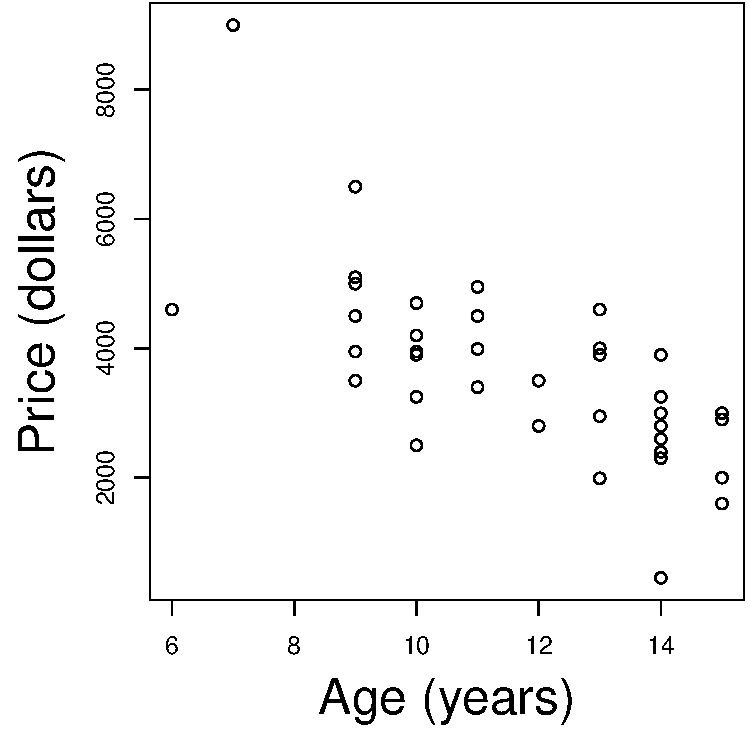
\includegraphics{figures/7-LinearModels-Figures/ageprice.pdf}
\end{center}
\end{slide}
\begin{slide}
\heading{Mitsubishi Example}

The age of a car is almost always known. Suppose that we want to predict the 
price of a randomly chosen 10 year old car. Then we can focus on the sample of
prices corresponding to cars with an age of 10 years. Graphically, this
corresponds to those observations within the vertical strip at {\tt age=10}.

Within this strip the average price is \$3750. If we now take a different
vertical strip corresponding to say, 14 year old cars then we get a different 
average price: \$2587. 
\textcolor{magenta}{Q: Find these values using R.}

If this process is repeated at several values of the age variable then we get
the following figure - a whole suite of mean values, conditional on the value of
age.
\textcolor{magenta}{Q: Write the R code to obtain the following plot.}

\end{slide}
\begin{slide}
\heading{Mitsubishi Example}

\begin{center}
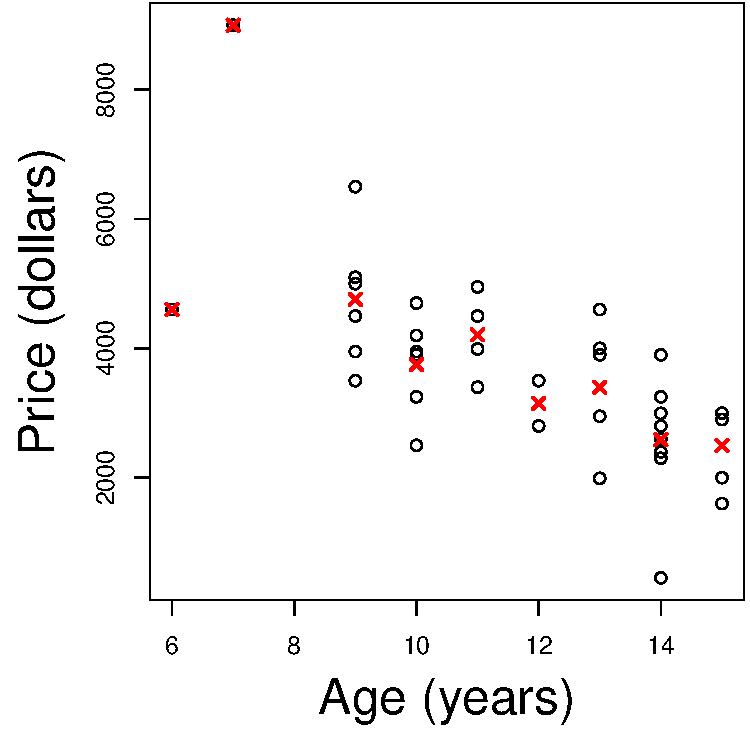
\includegraphics{figures/7-LinearModels-Figures/agepricex.pdf}
\end{center}
\end{slide}
\begin{slide}
\heading{Mitsubishi Example}

If we make the strips finer and finer then we get what is known as a regression
curve. This is defined to be the mean value of price for a given value of age.

One could think about repeating the calculations performed above based on 
the sample of prices of 10 year old cars to obtain a new prediction interval.
However, there are only five such observations, and therefore we would not
expect much accuracy. The situation is even worse for other car ages. There are
only 2 cars aged 12 years old, and no cars in the sample are 8 years old. How
do we use the data to predict prices of cars with these ages?

\end{slide}
\begin{slide}
\heading{Mitsubishi Example}

The usual approach is to model the regression curve. This means that we make 
some assumptions about what the regression curve look like. The curve in the 
above plot is approximately linear, so it may be reasonable to postulate the
{\it simple linear regression model} for these data and use this to predict
price from age.

Then the fitted linear regression model can be shown to be
$$\hat{\mbox{price}}=8452-409 \; {\tt age}$$

\end{slide}
\begin{slide}
\heading{Model formulation}
\begin{itemize}
\item In the Mitsubishi example, we say that {\tt age} is a \textcolor{blue}{\bf predictor} for 
{\tt price}. The variable {\tt age} is called the \textcolor{blue}{\bf predictor variable} and
{\tt price} is the \textcolor{blue}{\bf response variable}.

\item The usual generic notation for simple regression is
$$x=\mbox{ predictor variable}$$
$$y=\mbox{ response variable}$$

\item The prediction equation is
%
$$\hat{y}=\beta_0+\beta_1 x$$
\end{itemize}
\end{slide}
\begin{slide}
\heading{Model formulation}
\begin{itemize}

\item Therefore, if $y$ is any particular observation with corresponding $x$-value equal to 
$x$ then we can write 
$$y=\beta_0+\beta_1 x+\epsilon$$
where the {\it error } $\epsilon$ is given by
$$\epsilon=y-\hat{y}=y-(\beta_0+\beta_1 x)$$

\item Since we assume that $\beta_0+\beta_1 x$ is the average of the $y$s in the vertical strip about $x$, we will
have that
$$E(\epsilon)=0$$

\item Also $Var(y)$ in the vertical strip is equal to $\sigma^2$ so we have
$$Var(\epsilon)=\sigma^2$$

\item Finally because the observations in the vertical strips are normally distributed, we
have
$$\epsilon \sim N(0,\sigma^2)$$
\end{itemize}
\end{slide}
\begin{slide}
\heading{Model formulation}
\begin{itemize}

\item Thus we can write the simple linear regression model as
$$y=\beta_0+\beta_1 x+\epsilon, \quad \epsilon \sim N(0,\sigma^2).$$

\item Suppose we have $n$ observations, \\
$(x_1,y_1),\ldots,(x_n,y_n)$ from this model, then
$$y_i=\beta_0+\beta_1 x_i+\epsilon_i, i=1,\ldots, n$$
%
\item We assume further that the observations are collected independently of each other so that
the $\epsilon_i$ are independent. This means that a knowledge of one of the $e_i$ does not tell
us anything about the value of the other $e_i$s

\end{itemize}
\end{slide}
\begin{slide}
\heading{Linear Least Squares}
\begin{itemize}
\item In order to fit a straight line to a plot of points
$(x_i,y_i)$, where $i=1,\ldots,n$, the slope and intercept of the
line 
$$y =\beta_0+\beta_1x$$
must be found from the data in some manner

\item In order to fit a $p$-th order polynomial, $p+1$ coefficients must
be determined

\item Other functional forms besides linear and polynomial ones may be fit to 
data, and in order to do so, parameters associated with those forms must be
determined

\end{itemize}
\end{slide}
\begin{slide}
\heading{Linear Least Squares}
\begin{itemize}
\item The most common method for determining the parameters in curve-fitting
problems is the method of least squares

\item The idea is to minimize the sum of squared deviations of the predicted,
or {\it fitted} values, (given by the curve) from the actual observations.

\item Applying the method of {\bf least squares}, we choose the slope and
intercept of the straight line to minimize
$$S(\beta_0,\beta_1)=\sum_{i=1}^n (y_i-\beta_0-\beta_1x_i)^2$$
%
\item Note that $\beta_0$ and $\beta_1$ are chosen to minimize the sum of squared
vertical deviations, or prediction errors
%\end{itemize}
%\end{slide}
%\begin{slide}
%\heading{Linear Least Squares}
%\begin{itemize}

\item To find $\beta_0$ and $\beta_1$, we calculate
$$\frac{\partial S}{\partial\beta_0}=-2\sum_{i=1}^n(y_i-\beta_0-\beta_1x_i)$$
$$\frac{\partial S}{\partial\beta_1}=-2\sum_{i=1}^nx_i(y_i-\beta_0-\beta_1x_i)$$

\item Setting these partial derivatives equal to zero, we have that the minimizers
$\hat{\beta}_0$ and $\hat{\beta}_1$ satisfy
$$\sum_{i=1}^ny_i=n\hat{\beta}_0+\hat{\beta}_1\sum_{i=1}^nx_i$$
$$\sum_{i=1}^nx_iy_i=\hat{\beta}_0\sum_{i=1}^nx_i+\hat{\beta}_1\sum_{i=1}^nx_i^2$$

\item Solving for $\hat{\beta}_0$ and $\hat{\beta}_1$ , we obtain
$$\hat{\beta}_0=\frac{(\sum_{i=1}^nx_i^2)(\sum_{i=1}^ny_i)-(\sum_{i=1}^nx_i)(\sum_{i=1}^nx_iy_i)}{n\sum_{i=1}^nx_i^2-(\sum_{i=1}^nx_i)^2}$$

$$\hat{\beta}_1=\frac{n\sum_{i=1}^nx_iy_i-(\sum_{i=1}^nx_i)(\sum_{i=1}^ny_i)}{n\sum_{i=1}^nx_i^2-(\sum_{i=1}^nx_i)^2}$$

\end{itemize}
\end{slide}
\begin{slide}
\heading{Linear Least Squares}
\begin{itemize}

\item Functional forms more complicated than straight lines are often fit to data,
for example, when there are more than one predictor variables available, we may
fit a line of the form
$$y\approx \beta_0+\beta_1x_1+\beta_2x_2+\beta_3x_3$$
where $\beta_i$ could be estimated from data
%\end{itemize}
%\end{slide}
%\begin{slide}
%\heading{Linear Least Squares}
%\begin{itemize}
%

\item Or we may be able to fit functions of the following form to decay curves
$$f(t)=Ae^{-\alpha t}+Be^{-\beta t}$$
where the function $f$ is linear in the parameters $A$ and $B$ and nonlinear
in the parameters $\alpha$ and $\beta$,  
from data of the form $(y_i,t_i), i=1,\ldots,n$

\item When the function to be fitted is linear in the unknown parameters, the 
minimisation is relatively straightforward, since calculating partial derivatives
and setting them equal to zero produces a set of simultaneous linear equations
that can be solved in closed form. This special case is known as {\bf linear
least squares}
\end{itemize}
\end{slide}
\begin{slide}
\heading{Linear Least Squares}
\begin{itemize}

\item If the function to be fit is not linear in the unknown parameters, a system
of nonlinear equations must be solved to find the coefficients. Typically, the
solution cannot be found in closed form, so an iterative procedure must be used

\item For our purposes, the general formulation of the linear least squares 
problem is as follows: a function of the form
$$\begin{array}{ll}
&f(x_1,x_2,\ldots,x_{p-1})\\
=&\beta_0+\beta_1x_1+\beta_2x_2+\ldots+\beta_{p-1}x_{p-1}\end{array}$$
involving $p$ unknown parameters, $\beta_0,\beta_1,\ldots,\beta_{p-1}$
is to be fit to $n$ data points
$$\begin{array}{c}
y_1,x_{11},x_{12},\ldots,x_{1,p-1}\\
y_2,x_{21},x_{22},\ldots,x_{2,p-1}\\
\vdots\\
y_n,x_{n1},x_{n2},\ldots,x_{n,p-1}\\
\end{array}$$
%\end{itemize}
%\end{slide}
%\begin{slide} 
%\heading{Linear Least Squares}
%\begin{itemize}
%
\item The function $f(x)$ is called the {\bf linear regression} of $y$ on $x$

\item We will always assume that $p<n$, that is, there are fewer unknown 
parameters than observations

\item Fitting a straight line clearly follows this format

\item A quadratic can be fit in this way by setting $x_1=x$ and $x_2=x^2$

\item Many functions that are not initially linear in the unknowns can be put
into linear form by means of a suitable transformation

\end{itemize}
\end{slide}
\begin{slide}
\heading{Simple Linear Regression}
\begin{itemize}
\item Recall the simple linear regression model
$$y_i=\beta_0+\beta_1x_i+\epsilon_i, i=1,\ldots,n$$
where $\epsilon_i$ are independent random variables with 
$$E(\epsilon_i)=0, Var(\epsilon_i)=\sigma^2$$
the $x_i$s are assumed to be fixed

\item Under the simple linear regression model, the least squares estimates are
unbiased: 
$$E(\hat{\beta}_j)=\beta_j, j=0,1.$$
{\bf Proof: } In lecture.
\end{itemize}
\end{slide}
\begin{slide}
\heading{Simple Linear Regression}
\begin{itemize}

\item Note that here the proof does not depend on the assumption that $\epsilon_i$
are independent and have the same variance, only on the assumptions that the 
errors are additive and $E(\epsilon_i)=0$

\item From the simple linear regression model, $Var(y_i)=\sigma^2$ and
$Cov(y_i,y_j)=0$, where $i\neq j$, this makes the computation of the variances
of the $\hat{\beta}_j$s straightforward.

\item Under the assumptions of the simple linear regression model
$$Var(\hat{\beta}_0)=\frac{\sigma^2\sum_{i=1}^nx_i^2}{n\sum_{i=1}^nx_i^2-(\sum_{i=1}^nx_i)^2}$$
$$Var(\hat{\beta}_1)=\frac{n\sigma^2}{n\sum_{i=1}^nx_i^2-(\sum_{i=1}^nx_i)^2}$$

$$Cov(\hat{\beta}_0,\hat{\beta}_1)=\frac{-\sigma^2\sum_{i=1}^nx_i}{n\sum_{i=1}^nx_i^2-(\sum_{i=1}^nx_i)^2}$$

{\bf Proof:} In lecture.

\item We see that the variances of the slope and intercept depend on the $x_i$ and
on the error variances, $\sigma^2$

\item The $x_i$s are known, therefore to estimate the variance of slope and
intercept, we only need to estimate $\sigma^2$

\end{itemize}
\end{slide}
\begin{slide}
\heading{Simple Linear Regression}
\begin{itemize}

\item Since in the simple linear regression model, $\sigma^2$ is just the expected
squared deviation of th $y_i$s from the line $\beta_0+\beta_1x_i$, it is 
natural to base an estimate of $\sigma^2$ on the average squared deviations
of the data about the fitted line, we define the {\bf residual sum of
squares (RSS)} to be
$$RSS=\sum_{i=1}^n(y_i-\hat{\beta}_0-\hat{\beta}_1x_i)^2$$
and
$$S^2=\frac{RSS}{n-2}$$
is an unbiased estimator of $\sigma^2$
\end{itemize}
\end{slide}
\begin{slide}
\heading{Simple Linear Regression}
\begin{itemize}

\item The divisor $n-2$ is used rather than $n$ because two parameters
have been estimated from the data, giving $n-2$ degrees of freedom

\item The variances of $\hat{\beta}_0$ and $\hat{\beta}_1$ are thus estimated
by replacing $\sigma^2$ by $S^2$, yielding estimates that we will denote
$s^2_{\hat{\beta}_0}$ and $s^2_{\hat{\beta}_1}$.

\item If the errors $\epsilon_i$ are independent normal random variables, then
the estimated slope and intercept, being linear combinations of independent 
random variables, are normally distributed as well

\end{itemize}
\end{slide}
\begin{slide}
\heading{Simple Linear Regression}
\begin{itemize}
\item More generally, if the $\epsilon_i$ are independent and the $x_i$ satisfy 
certain assumptions, a version of the central limit theorem implies  that, for 
large $n$, the estimated slope and intercept are approximately normally 
distributed

\item The normality assumption, or its approximation makes possible the 
construction of confidence intervals and hypothesis tests. It can be shown that
$$\frac{\hat{\beta}_i-\beta_i}{s_{\hat{\beta}_i}}\sim t_{n-2}$$
which implies that the $t$ distribution can be used for confidence intervals
and hypothesis tests.
\end{itemize}
\end{slide}
\begin{slide}
\heading{Mitsubishi Example:}

For the Mitsubishi price/age data, using the R commands 

\begin{Verbatim}[commandchars=\\\{\}]
\textcolor{magenta}{ > # Question: }
\textcolor{magenta}{ > # Write down the code}
\textcolor{magenta}{ > # Hint: use `lm' function}
\end{Verbatim}
%
%> mitsub.lm <- lm(price ~ age, data = mitsub)
%> summary(mitsub.lm)
%


gives that the estimates of the coefficients are
$$\hat{\beta}_0=8451.591 \quad \hat{\beta}_1=-409.2175$$

and the residual variance is
$$\hat{\sigma}^2=1045^2$$

The R output is 

{\small
\begin{verbatim}
> summary(lm(price ~ age))

Call:
lm(formula = price ~ age)

Residuals:
    Min      1Q  Median      3Q     Max 
-2272.5  -504.8  -122.5   568.2  3411.9 

Coefficients:
            Estimate Std. Error t value Pr(>|t|)    
(Intercept)  8451.59     840.05  10.061 3.89e-12 ***
age          -409.22      69.79  -5.863 9.62e-07 ***
---
Signif. codes:  0 `***' 0.001 `**' 0.01 `*' 0.05 `.' 0.1 ` ' 1 

Residual standard error: 1045 on 37 degrees of freedom
Multiple R-Squared: 0.4816,     Adjusted R-squared: 0.4676 
F-statistic: 34.38 on 1 and 37 DF,  p-value: 9.618e-07 

\end{verbatim}}
\end{slide}
\begin{slide}
\heading{Mitsubishi Example:}

Hence the fitted line is 
$$\hat{\mbox{price}}=8451.59-409.22 \mbox{ age}.$$

The estimated price of new Mitsubishi Sigma cars ({\tt age =0}) is \$8451.59

The estimated depreciation rate of Mitsubishi Sigma cars is \$409.22 per year

The standard error of the intercept, $s_{\hat{\beta}_0}=840.05$. A 95\% confidence
interval for the intercept, $\beta_0$ based on the $t$ distribution with 37 df is
$$\hat{\beta}_0\pm t_{37}(0.025)s_{\hat{\beta}_0} \Longrightarrow (6748.897, 10153.10).$$
\end{slide}
\begin{slide}
\heading{Mitsubishi Example:}

Similarly, a 95\% confidence interval for the slope $\beta_1$, is
$$\hat{\beta}_1\pm t_{37}(0.025)s_{\hat{\beta}_1} \Longrightarrow (-550.628, -267.8120).$$

To test the null hypothesis $H_0:\beta_0=0$, we would use the $t$ statistic
$\hat{\beta}_0/s_{\hat{\beta}_0}=10.061$. The hypothesis would be rejected at significance level
$\alpha=0.05$, there is strong evidence that the intercept is non-zero.

\textcolor{magenta}{Q: Write the code that returns the predicted price of a 10 years old car (Hint: use the {\tt predict} function)}

\textcolor{magenta}{Q: Write the code that produces the graph below (Hint: use the {\tt abline} function)}
\begin{center}
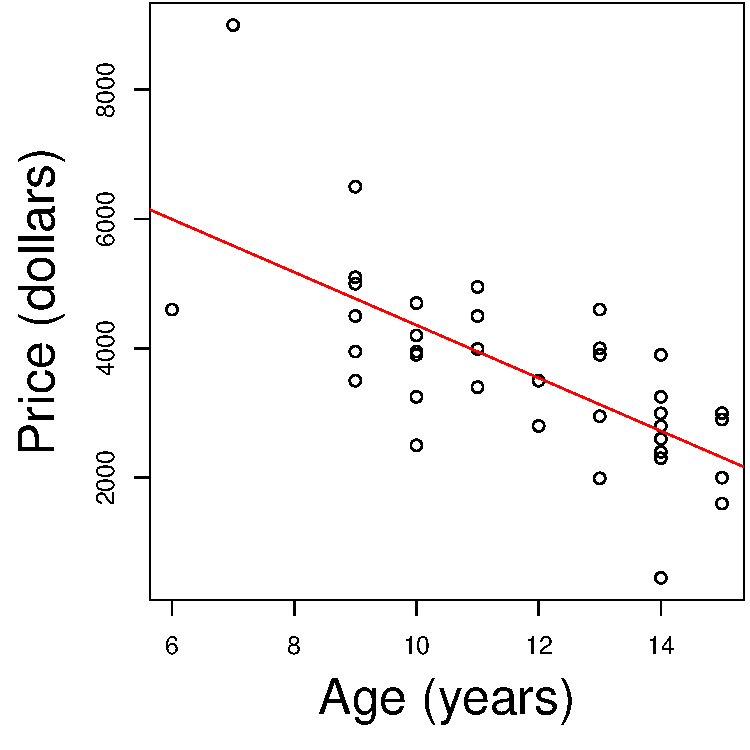
\includegraphics[width=0.5\textwidth]{figures/7-LinearModels-Figures/mitsub_reg.pdf}
\end{center}

\end{slide}


\begin{slide}
\heading{Maximum likelihood estimators in simple linear regression model}

MLEs of $\beta_0$, $\beta_1$ and $\sigma^2$ under
normality assumptions?

Maximizing the likelihood is equivalent to maximizing
the log-likelihood:  if $L_1<L_2$ are values
of the likelihood function for two different points
in parameter space, $\log(L_1)<\log(L_2)$.

Likelihood for single observation $y_i$:
\begin{eqnarray*}
   & &   \frac{1}{\sqrt{2\pi\sigma^2}}
       \exp\left(-\frac{1}{2\sigma^2}(y_i-\beta_0-\beta_1 x_i)^2\right)
\end{eqnarray*}

Independent errors, full likelihood:
\begin{eqnarray*}
  & & \prod_{i=1}^n
       \frac{1}{\sqrt{2\pi\sigma^2}}
       \exp\left(-\frac{1}{2\sigma^2}(y_i-\beta_0-\beta_1 x_i)^2\right) \\
        & = & (2\pi\sigma^2)^{-\frac{n}{2}}
\exp\left(-\frac{1}{2\sigma^2}\sum_{i=1}^n(y_i-\beta_0-\beta_1
x_i)^2\right).
\end{eqnarray*}
%
%\end{slide}
%\begin{slide}
%\heading{Maximum likelihood estimators in simple linear regression model}
%
Log likelihood:
%
\begin{eqnarray*}
&  &
    -\frac{n}{2}\log(2\pi\sigma^2)-\frac{1}{2\sigma^2}\sum_{i=1}^n
     (y_i-\beta_0-\beta_1 x_i)^2  \\
   & = &
    -\frac{n}{2}\log(2\pi)-\frac{n}{2}\log(\sigma^2)  
%    \\
%&  &   
-\frac{1}{2\sigma^2}\sum_{i=1}^n
     (y_i-\beta_0-\beta_1 x_i)^2
\end{eqnarray*}

Regardless of $\sigma^2$, the above is maximized with respect to
$\beta_0$ and $\beta_1$ by minimizing
\begin{eqnarray*}
   \sum_{i=1}^n(y_i-\beta_0-\beta_1 x_i)^2.
\end{eqnarray*}

$\Longrightarrow$ Least squares and maximum likelihood estimators of $\beta_0$,
$\beta_1$ coincide

\end{slide}
\begin{slide}
\heading{Maximum likelihood estimator of error variance}

Maximum likelihood estimator of $\sigma^2$?
%
\begin{eqnarray*}
  & &   \frac{\partial}{\partial \sigma^2}\left(
         -\frac{n}{2}\log\sigma^2 -\frac{1}{2\sigma^2}
         \sum_{i=1}^n (y_i-\beta_0-\beta_1 x_i)^2\right) \\
  & = &
        -\frac{n}{2\sigma^2}+\frac{1}{2\sigma^4} \sum_{i=1}^n(y_i-\beta_0
          -\beta_1 x_i)^2.
\end{eqnarray*}

Set to zero, write $\hat{\sigma}^2$ for MLE, substitute $\hat{\beta}_0$ and
$\hat{\beta}_1$ for $\beta_0$ and $\beta_1$,
%\begin{eqnarray*}
%   \frac{n}{2\hat{\sigma}^2} & = &
%\frac{1}{2\hat{\sigma}^4}\sum_{i=1}^n(y_i-\hat{\beta}_0-\hat{\beta}_1 x_i)^2
%\end{eqnarray*}
which gives
\begin{eqnarray*}
   \hat{\sigma}^2 & = & \frac{1}{n}\sum_{i=1}^n (y_i-\hat{\beta}_0-\hat{\beta}_1 x_i)^2.
\end{eqnarray*}

\end{slide}


\end{document}


